% A simple template for LaTeX documents
% 
% To produce pdf run:
%   $ pdflatex paper.tex 
%


\documentclass[12pt]{article}

% Begin paragraphs with new line
\usepackage{parskip}  

% Change margin size
\usepackage[margin=1in]{geometry}   

% Graphics Example:  (PDF's make for good plots)
\usepackage{graphicx}               
% \centerline{\includegraphics{figure.pdf}}

% subfigures, side by side
\usepackage{subcaption}

% hyperlinks
\usepackage{hyperref}

% Blocks of code
\usepackage{listings}
\lstset{basicstyle=\ttfamily, title=\lstname}
% Insert code like this. replace `plot.R` with file name.
% \lstinputlisting{plot.R}

% Monospaced fonts
%\usepackage{inconsolata}
% GNU \texttt{make} is a nice tool.

% Supports proof environment
\usepackage{amsthm}

% Allows writing \implies and align*
\usepackage{amsmath}

% Allows mathbb{R}
\usepackage{amsfonts}

% Numbers in scientific notation
% \usepackage{siunitx}

% Use tables generated by pandas
\usepackage{booktabs}

% Allows umlaut and non ascii characters
\usepackage[utf8]{inputenc}

% Insert blank pages
\usepackage{afterpage}
%\afterpage{\null\newpage}

% norm and infinity norm
\newcommand{\norm}[1]{\left\lVert#1\right\rVert}
\newcommand{\inorm}[1]{\left\lVert#1\right\rVert_\infty}

% Statistics essentials
\newcommand{\iid}{\text{ iid }}
\newcommand{\Exp}{\operatorname{E}}
\newcommand{\Var}{\operatorname{Var}}
\newcommand{\Cov}{\operatorname{Cov}}


%%%%%%%%%%%%%%%%%%%%%%%%%%%%%%%%%%%%%%%%%%%%%%%%%%%%%%%%%%%%

\begin{document}

\title{Parallel Computing Through Code Analysis}
\date{\today}
\author{Clark Fitzgerald}
\maketitle

\begin{abstract}

    Conventional systems for parallel programming require users to modify
    existing code to take advantage of a platform's computational
    capabilities, which may include multiprocessing or Graphical Processing
    Units (GPU)s. In this proposal we consider code analysis methods to
    detect the potential for parallel execution. The results of the
    analysis can then be used to rewrite and execute semantically
    equivalent parallel instructions, without requiring the user to modify
    their original code.  We consider a motivating case study analyzing the
    operating characteristics California's highway traffic sensor stations
    on hundreds of gigabytes of traffic sensor data.

\end{abstract}

This is a prospectus for distribution to the committee for PhD
Qualifying Exam in June 2017.

\section{Code, Data, Platform}
%%%%%%%%%%%%%%%%%%%%%%%%%%%%%%%%%%%%%%%%%%%%%%%%%%%%%%%%%%%%

\begin{figure}
\centering
\includegraphics[width=.5\linewidth]{workflow}
\caption{Given sequential code and a description of the data we seek
    a modified computational parallel plan tailored to a specific platform.}
\label{fig:workflow}
\end{figure}

Figure \ref{fig:workflow} shows the high level goal.
\textbf{Code} is a script to be executed.
\textbf{Data} could be data in memory, single or multiple files, a
memory-mapped file, a database, a parallel file system, etc.
\textbf{Platform} is the computing setup, such as a laptop with 4 cores, a
Spark cluster, or a server with 2 GPUs and a high bandwidth connection. The combination
of (Code, Data, Platform) dictates what strategies should be used for
efficient evaluation. Given these three components, our goal is to analyze the
code, potentially reorganizing it for efficient execution on the data and
platform. This doesn't mean that the system is inventing new algorithms on
the fly. But it should be capable of tuning existing parameters to the
system at hand. An example of a parameter to be tuned is the chunk size
$n_j$ as described in \ref{section:sequential}.

This project is in the spirit of compiling R, since it treats R code as
a set of high level directions, and it potentially generates alternative
code for execution \cite{lang2014enhancing}.

\section{Motivating Example}
%%%%%%%%%%%%%%%%%%%%%%%%%%%%%%%%%%%%%%%%%%%%%%%%%%%%%%%%%%%%
\label{sec:pems}

The California Department of Transportation collects traffic data through
sensors embedded in highways. The sensors measure three quantities: count
of passing vehicles, time during which a vehicle is directly above the
sensor (occupancy), and average velocity \cite{jia2001pems}.  Every thirty
seconds they produce a new data point. $43,680$ sensors in California
measuring 3 parameters multiplied by $(2 \times 60 \times 24)$ measurements
per day results in 377 million new data points per day.  This raw data is
organized into files grouped by (day, district), and is available for
public download.  As an analyst I would like to model velocity as a
function of occupancy for each sensor. This relationship is called the
``fundamental diagram'' within traffic engineering, because it captures the
operating characteristic of this section of road
\cite{daganzo1997fundamentals}. Once these fundamental diagrams have been
modeled for each station they can be used to understand how other road
characteristics such as on ramps and off ramps affect the flow of traffic.

Robust regression can be used to fit the fundamental diagram, approximating
the integer programming approach to minimize the L1 norm as in
\cite{li2011fundamental}.  From the R language this can be done easily and
efficiently, for example with the \texttt{rlm} (robust linear model)
function in the MASS package \cite{venables2013modern}:

\begin{verbatim}
fit1 = rlm(velocity ~ occupancy, data = station1)
\end{verbatim}

However, the size and organization of the data makes the task much more
difficult.  I've downloaded a subset of the data consisting of measurements
in the San Francisco Bay Area for part of 2016.  It would be easier to
perform the regression if the data were organized in files for each sensor
rather than in files for each day.  One approach then is to reorganize the
data on disk into this file structure. I did this using a simple single
threaded R program, and it took 23 hours to run on 134 GB of data.
Throughput for a conventional hard disk is around 100
MB/s\footnote{Parallel filesystems will increase throughput}, so a lower
bound for reading then writing this reorganized data is approximately $2 *
134000 / 100$ seconds, or 45 minutes. The naive code is 30 times slower
than this. So small inefficiencies add up.

Another drawback is that it requires very specific instructions to
reorganize the data for computations grouped by station. Any parallel
programming will make this even more specific to the data and platform. The
following R code captures the desired semantics:

\begin{verbatim}
by(data, INDICES = station, FUN = piecewise_rlm)
\end{verbatim}

This says group \texttt{data} by \texttt{station}, and apply the
function \texttt{piecewise\_rlm} to each group.

What if we had a system that could inspect the idiomatic R code above that
works on small data sets, and then automatically take steps to scale and to
parallelize the operations? It could also tune them for the specifics of
the system and the data. This is what we're working towards.


\section{Simple Example}
%%%%%%%%%%%%%%%%%%%%%%%%%%%%%%%%%%%%%%%%%%%%%%%%%%%%%%%%%%%%

% Duncan:
% Come up with concrete and realistic examples.  Show how you would do things
% differently for different computational platform Go through this explicitly
% by hand to show the "ideal" transformed code (keep high level) Identify how
% you might identify these programmatically and what are some of the
% challenges

Now we use a simple example to see exactly what translating code might look
like.  Consider computing the mean,

\begin{equation}
    \bar{x} = \frac{1}{n} \sum_{i = 1}^n x_i
\label{eq:mean}
\end{equation}

where the $x_i$'s are
i.i.d. $\sim N(0, 1)$.  In R this code is written:

\begin{verbatim}
xbar = mean(rnorm(n))
\end{verbatim}

To evaluate this R will first build an intermediate vector $x = (x_1,
\dots, x_n)$ and then compute the mean. Eventually that unreferenced
intermediate vector will be garbage collected.
Execution time increases
linearly with $n$. Once $n$ becomes large
enough this vector will no longer fit into available physical memory, so
the operating system will use swap space. On a machine with 8 GB memory
this happens when $O(n) = 10^9$, causing the execution time
to increase by an order of magnitude, roughly from 1 minute to 15
minutes. Once $n$ exceeds memory and swap space R will not be able to allocate a
large enough object, and the computation will fail.

Now we consider alternative ways to execute this code.  Most rely on
splitting the sum into $p$ partial sums with $n_j$ terms each and then rewriting
Equation \ref{eq:mean} as a weighted mean.

\begin{equation}
    \bar{x} = \frac{1}{n} \sum_{j = 1}^p \sum_{i = 1}^{n_j} x_{ij}
    = \sum_{j = 1}^p \frac{n_j}{n} \bar{x}_j
\label{eq:mean_partial}
\end{equation}

It's important to correctly handle the cases when $n$ is not divisible by $p$
and the computation / data cannot be evenly split. For simplicity in the
examples below, suppose that they can be split evenly so $n_j$ is the same
for all $j$.

\subsection{Sequential Execution}
\label{section:sequential}

Equation \ref{eq:mean_partial} can be directly translated into R code as
follows:

\begin{verbatim}
partial_means = replicate(p, mean(rnorm(n_j)))
xbar = mean(partial_means)
\end{verbatim}

This code does not run in parallel, but it does use the same functional
programming patterns as parallel code. If $M$ is the size of physical memory in
bytes then this code is high performance in the sense
that execution time will continue to be linear while $n < O(M^2)$, just
as it was for small $n < O(M)$. It can also be modified to handle
arbitrarily large $n$. This is because \texttt{replicate()} runs
sequentially, so the memory footprint can be bounded since the intermediate
vectors will be of length $n_j$. 

What aspects of the code changed? In the initial code the user
supplied $n$, and it remained to choose $p$ and $n_j$.

\subsection{SNOW Cluster}

Clusters created by SNOW, a Simple Network Of Workstations,
consist of independent worker R processes created by a manager process. The
processes communicate over network sockets, and they may be on one or many
physical machines.  This is the type of cluster used by partools and
Software Alchemy \cite{R-partools} \cite{matloff2014software}.  The code
pattern is similar to \ref{section:sequential}; the \texttt{replicate()}
becomes \texttt{clusterEvalQ()}:

\begin{verbatim}
library(parallel)
p = detectCores()
n_j = n / p
cluster = makeCluster(p)
clusterExport(cluster, "n_j")
partial_means = unlist(
    clusterEvalQ(cluster, mean(rnorm(n_j))))
xbar = mean(partial_means)
\end{verbatim}

The manager sends the code  \texttt{mean(rnorm(n\_j))} to each worker in
the cluster to be evaluated in parallel. Given an existing cluster this is
very efficient, since we are sending a few bytes of code over the network
and then returning a single number. This parallel model is useful in
statistics when doing independent simulations.

\section{Design Considerations}
%%%%%%%%%%%%%%%%%%%%%%%%%%%%%%%%%%%%%%%%%%%%%%%%%%%%%%%%%%%%

\subsection{Overhead}

Many of the performance characteristics of the different platforms can be
understood in terms of the overhead to set them up, and then the latency
and bandwidth for when data must be transferred.  If the data is ``small
enough'' then performance will be acceptable regardless of how well the
platform is utilized or how efficient the code is. Conversely, if the data
is ``large enough'' then \emph{everything} matters, since small
inefficiencies will be magnified when they occur millions of times, as in
Section \ref{sec:pems}.  Therefore the focus here is on problems which take longer
to run. A priori one doesn't even know if it's possible to run code more
efficiently in parallel, due to the overhead.

\begin{figure}
\centering
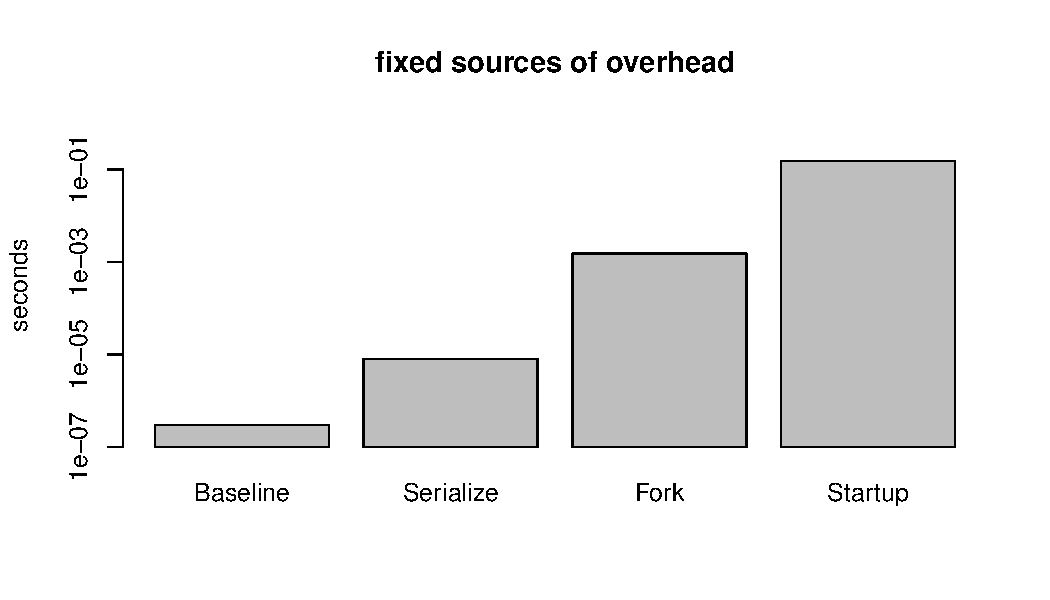
\includegraphics[width=.8\linewidth]{compute_times/overhead}
\caption{Simple function calls take less than a microsecond. Launching a
    new R interpreter takes hundreds of milliseconds, which is relatively expensive.}
\label{fig:overhead}
\end{figure}

Figure \ref{fig:overhead} compares the relative fixed sources of overhead to
consider with parallel programming. The evaluation of the following simple
function captures the basic overhead associated with an interpreted
language like R:
\begin{verbatim}
twox = function(x) 2*x
\end{verbatim}
Every call to this function will incur a fixed overhead that is a couple
hundred nanoseconds. Vectorization refers to passing longer vectors to the
function to amortize this fixed cost. For example, if $x$ is an integer
vector of length 1 then the overhead takes 2 orders of magnitude more time
than the actual computation. However, if $x$ is of length 1500 then this
overhead accounts for only 10 percent of the total execution time, so the
fixed cost has been amortized.

Each platform has constraints which may include:

\begin{itemize}
    \item number of cores available
    \item network bandwidth
    \item disk IO speed
    \item available memory
\end{itemize}

We can control:

\begin{itemize}
    \item number of processor cores to use
    \item size of each chunk
    \item which functions to combine in one processing step
\end{itemize}

\subsection{Interfaces}

Parallel programming in pure R (not at the C level) can be understood in
terms of a layered architecture. The foundational \textbf{System Layer}
provides the basic interfaces used by any programming language. The
\textbf{R Layer} consists of packages which adapt the basic interfaces for
use specifically in R. The packages in the \textbf{User Layer} are meant to
simplify parallel programming, or they are for applications with specific
use cases.  Here are a few examples of packages at each layer:

\begin{itemize}
\item User Layer: foreach, future, partools, ddR, biganalytics, RevoScaleR
\item R layer: SNOW, multicore, parallel, bigmemory, Rmpi
\item System Layer: processes, *NIX fork(), memory maps, network sockets,
    MPI
\end{itemize}

Currently, users write code using packages from the User Layer or the R
Layer. Code analysis potentially can allow us to skip these layers, and
instead write the same base R code which will run in serial as in parallel.
This is appealing for a few reasons. Base R is stable, so users can write
the same working code without committing to a particular package or
architecture. If the code runs on a different system or with a different
data set then one can automatically generate code to run more efficiently
on that system.

%TODO: expand
Some of the work here may mean enhancing the capabilities of these
intermediate layers. For example, a file based sort usable from R allows
``group by'' and facilitiates streaming applications.

\section{Code Analysis}
%%%%%%%%%%%%%%%%%%%%%%%%%%%%%%%%%%%%%%%%%%%%%%%%%%%%%%%%%%%%

Static code analysis is integral to this approach, and we build on the 
CodeDepends package \cite{R-CodeDepends}.

\subsection{Expression Dependency Graphs}

TODO: Copy stuff from last quarter here and relate it to Pablo's example.

Steps:

\begin{itemize}
    \item Parse the code, gathering dependency information
    \item Identify points to parallelize
    \item Speculatively evaluate some expressions (after checking for side
        effects) to estimate how long they'll
        take
    \item Determine if preprocessing of the data is required
    \item Generate code that will run in parallel on that platform
    \item Estimate total time required to run
\end{itemize}

\subsection{Interesting parts of code}

Three types of functions in R are of special interest when doing parallel
computation: apply functions, vectorized
functions, and reduce functions.

Apply functions are higher order functions that include an implicit loop
which can be parallelized. They include \texttt{lapply, apply, sapply,
vapply, Map, mapply, by, tapply, outer, replicate}, and follow the basic
form of an embarrassingly parallel map-reduce problem.

Vectorized functions apply functions elementwise, for example arithmetic
operators \texttt{+, -, *, /}.

TODO: Relate vectorization and loop fusion

The general form of the \texttt{Reduce()} function in R collapses elements
into a single result by calling a function $f()$ repeatedly on the
elements. For example \texttt{Reduce(`+`, 1:4)} is equivalent to 
\texttt{(((1 + 2) + 3) + 4)}. More common examples that can be written this
way include \texttt{min, max, mean, sum, prod}. Since we're computing on
large data sets numerically stable algorithms should be used here, ie.
Kahan summation \cite{Robey2011217}.

\subsection{Related Technologies}

Related technologies include Theano, tensorflow, and arrayfire. Theano and
tensorflow have the user build computation graphs which are then executed in
an efficient way based on the available architecture. They are more
tailored to linear algebra / numerical computing, and are often used for
components of neural networks.

\bibliographystyle{plain}
\bibliography{../citations,../Rpackages} 

\end{document}
